\documentclass[11pt,letterpaper]{article}

\usepackage[utf8]{inputenc}
\usepackage[T1]{fontenc}
\usepackage{lmodern}
\usepackage[spanish,es-tabla,es-noshorthands]{babel}
\usepackage[margin=2.5cm]{geometry}
\usepackage{amsmath}
\usepackage{graphicx}
\usepackage{booktabs}
\usepackage{tabularx}
\usepackage{float}
\usepackage{caption}
\usepackage{pgfplots}
\pgfplotsset{compat=1.18}
\usepackage[hidelinks]{hyperref}

\captionsetup{font=small, labelfont=bf}
\setlength{\parskip}{0.4em}

\pgfplotsset{
  barras/.style={
    ybar, bar width=9pt, width=0.48\textwidth, height=4.8cm,
    ymin=0, enlarge x limits=0.25, enlarge y limits={upper, value=0.25},
    xtick={0,1,2}, xticklabels={Normal,Semana Santa,Navidad},
    tick label style={font=\footnotesize}, ylabel style={font=\footnotesize},
    nodes near coords={\pgfmathprintnumber[fixed, precision=1]{\pgfplotspointmeta}},
    every node near coord/.append style={font=\tiny, rotate=90, anchor=west},
  },
  actual/.style={fill=gray!40, draw=gray!70!black},
  algoritmo/.style={fill=blue!55!black, draw=blue!40!black},
}

\begin{document}
\spanishplainpercent

\begin{titlepage}
  \centering
  {\large Universidad del Valle de Guatemala\par}
  Facultad de Ingeniería\par
  Ciencia de la Computación y Tecnologías de la Información\par
  CC2017 -- Modelación y Simulación\par
  Ciclo 2, 2026\par
  \vspace{5cm}
  {\LARGE\bfseries Práctica 4\par}
  \vspace{0.5cm}
  {\Large Rutas de reparto y tamaño de flota\\ en Logística del Valle\par}
  \vspace{5cm}
  {\large Juan Fernando Menéndez Guerra -- 17444\par}
  \vfill
  {\today\par}
\end{titlepage}

\section{Introducción}

Logística del Valle distribuye productos de farmacia desde una bodega, identificada como N01, hacia cuatro zonas de entrega: N08, N19, N34 y N40. Los conductores siguen recorridos que aprendieron hace años y la gerencia no sabe si esas rutas siguen siendo convenientes, ni si los ocho vehículos con los que cuenta la empresa alcanzan en las temporadas de mayor demanda, cuando el promedio de pedidos sube de cuatro por hora a seis en Semana Santa y a diez en Navidad.

Para responder estas preguntas se construyó un grafo dirigido a partir de la matriz de tiempos de viaje proporcionada por la empresa, se verificaron las rutas de las hojas de despacho y se calcularon rutas alternativas con el algoritmo de Dijkstra. Con esas rutas se desarrolló una simulación de eventos discretos de la jornada de trabajo, en la que se comparan dos políticas, mantener las rutas actuales o usar las del algoritmo, en los tres escenarios de demanda y con distintos tamaños de flota. El modelo se implementó en Go junto con una aplicación web local, en la que se pueden cambiar los parámetros de la simulación, modificar o cerrar tramos y observar cómo cambian las rutas y los resultados.

\section{Formulación del problema}

\subsection{Objetivos}

\paragraph{Objetivo general.} Evaluar si las rutas y la flota actuales de Logística del Valle permiten cumplir con entregas puntuales en temporada normal y en temporada alta, y proponer cambios de rutas y de flota sustentados en un modelo de grafos y en una simulación de eventos discretos.

\paragraph{Objetivos específicos.}
\begin{enumerate}
  \item Construir el grafo dirigido de la red a partir de la matriz de tiempos y comprobar si las rutas registradas son válidas de ida y de regreso.
  \item Calcular, con un algoritmo de rutas más cortas, la ida y el regreso para cada destino y compararlos con las rutas actuales.
  \item Simular la llegada y atención de pedidos para medir el efecto de cambiar las rutas en los escenarios normal, Semana Santa y Navidad.
  \item Determinar a partir de qué demanda la flota de ocho vehículos deja de ser suficiente y cuántos vehículos se necesitarían en cada escenario.
\end{enumerate}

\subsection{Datos proporcionados}

\begin{itemize}
  \item Matriz de adyacencia de $40\times 40$ con los tiempos de viaje en minutos. Cada fila es un origen y cada columna un destino; el 0 de la diagonal identifica el mismo punto y una celda vacía indica que no hay conexión directa. La matriz puede ser asimétrica porque algunas calles son de un solo sentido.
  \item La bodega N01, los destinos N08, N19, N34 y N40 y la ruta de ida de las hojas de despacho para cada destino. Según las hojas, el vehículo regresa por el mismo camino en sentido inverso.
  \item La recepción de pedidos dura ocho horas, con un promedio de 4, 6 y 10 pedidos por hora en los escenarios normal, Semana Santa y Navidad. Los cuatro destinos reciben aproximadamente la misma proporción de pedidos.
  \item La empresa tiene ocho vehículos. Cada uno lleva un solo pedido y debe volver a N01 antes de atender otro; si no hay vehículos disponibles, los pedidos esperan en orden de llegada.
  \item Una entrega es puntual si se completa en 75 minutos o menos desde que se recibe la solicitud, incluido el tiempo de espera.
\end{itemize}

\subsection{Decisiones que se evalúan}

La primera decisión es la política de rutas: mantener los recorridos de las hojas de despacho o cambiarlos por los que recomienda el algoritmo. La segunda es el número de vehículos, que se evalúa para cada escenario de demanda. La tercera es cómo responder a un incidente vial, cuando un tramo se congestiona o se cierra, y cuánto afecta ese cambio a cada política.

\subsection{Supuestos del modelo}

\begin{itemize}
  \item Los tiempos de viaje son los de la matriz y no cambian con la hora del día ni de un viaje a otro.
  \item La carga en la bodega y la entrega al cliente no consumen tiempo: la entrega ocurre al llegar al destino.
  \item Los pedidos llegan según un proceso de Poisson con tasa constante durante la recepción, y cada destino tiene probabilidad $1/4$.
  \item Al iniciar la jornada todos los vehículos están libres en N01. No se consideran averías, descansos ni cambios de turno, y los vehículos pueden seguir trabajando después de las ocho horas.
  \item Si hay varios vehículos libres sale el que lleva más tiempo esperando. Como los vehículos son iguales, esta regla no cambia los resultados de los pedidos.
  \item Con la política actual, si un tramo de la ruta está cerrado, el conductor toma el desvío más corto entre los extremos de ese tramo y después sigue su ruta habitual.
  \item El tiempo adicional se mide desde el cierre de la recepción hasta la última entrega. La utilización se calcula hasta que el último vehículo vuelve a la bodega.
\end{itemize}

\section{Grafo generado}

La matriz se interpretó como un grafo dirigido y ponderado $G=(V,A,w)$ con $|V|=40$. Existe el arco $(i,j)$ cuando la celda de la fila $i$ y la columna $j$ tiene un valor, y su peso $w(i,j)$ es el tiempo de viaje en minutos. Una calle de doble sentido aparece como dos arcos, $(i,j)$ y $(j,i)$, que pueden tener tiempos distintos, y una calle de un solo sentido como un único arco. En el programa la red se guarda igual que la matriz, en un arreglo de $40\times 40$ en el que $-1$ indica que no hay conexión. Al leer el archivo hay que tener cuidado con las celdas vacías: si se tomaran como cero, aparecerían tramos sin costo entre puntos que no están conectados.

La red tiene 144 arcos. Hay 63 pares de nodos conectados en ambos sentidos; en 14 de ellos el tiempo cambia según el sentido, por ejemplo N04$\rightarrow$N11 tarda 9 minutos y N11$\rightarrow$N04 tarda 5. Los 18 arcos restantes son calles de un solo sentido, entre ellas N01$\rightarrow$N17, N02$\rightarrow$N18, N11$\rightarrow$N13, N17$\rightarrow$N26 y N18$\rightarrow$N26. Desde cualquier punto se puede llegar a cualquier otro, de modo que el grafo es fuertemente conexo.

La Figura~\ref{fig:grafo} muestra el grafo dibujado con Graphviz (Gansner y North, 2000) a partir de un archivo DOT que genera el programa. Como no se proporcionó un mapa, los nodos se acomodaron en una cuadrícula de cinco filas y ocho columnas según su numeración, porque casi todos los tramos unen nodos con números consecutivos o separados por ocho. La posición de los nodos no representa su ubicación geográfica. Los sentidos de circulación se representan con el color y las flechas, y los tiempos con la etiqueta de cada tramo.

\begin{figure}[H]
  \centering
  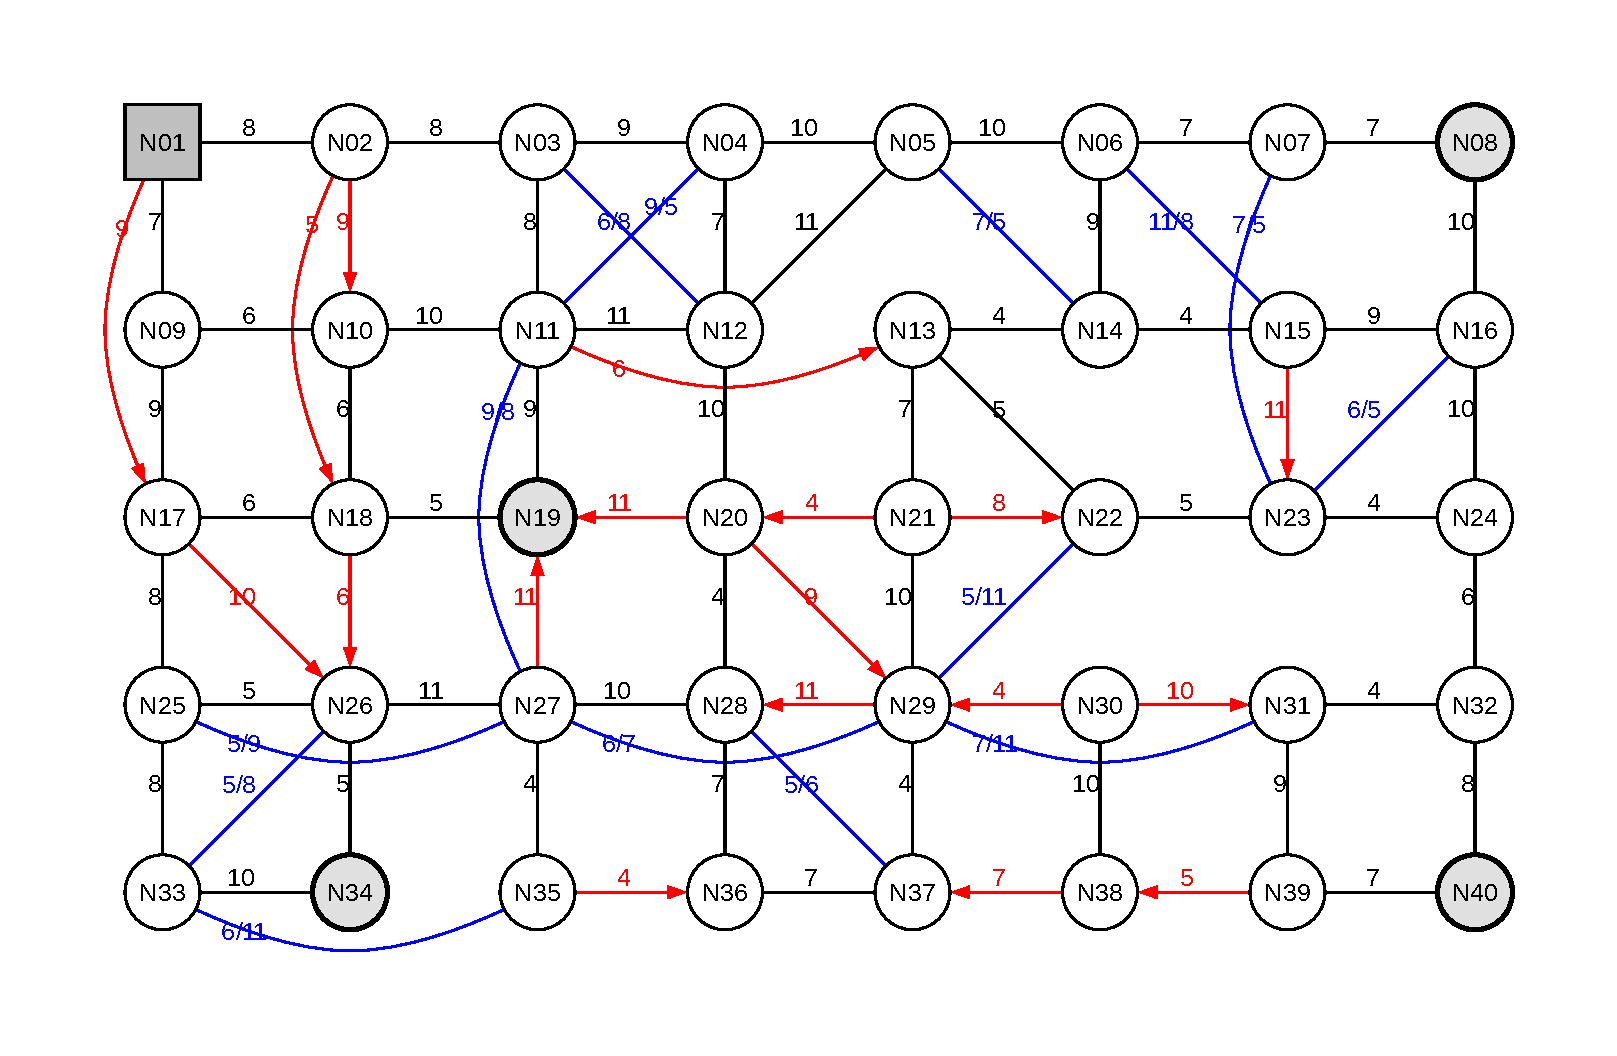
\includegraphics[width=\textwidth]{figuras/grafo.pdf}
  \caption{Grafo de la red. Negro: doble sentido con el mismo tiempo. Azul: doble sentido con tiempos distintos; la etiqueta $a/b$ indica el tiempo del nodo de menor número al de mayor número ($a$) y el del sentido contrario ($b$). Rojo con flecha: un solo sentido. El rectángulo es la bodega y los círculos de borde grueso son los destinos.}
  \label{fig:grafo}
\end{figure}

Para validar una ruta se recorre su secuencia de nodos, se comprueba que exista cada arco y se suman sus tiempos. El regreso se valida de la misma forma con la secuencia invertida, porque un tramo que existe de ida puede no existir de vuelta. La Tabla~\ref{tab:actuales} resume el resultado. Las cuatro rutas son válidas en ambos sentidos y tardan lo mismo de ida que de regreso, ya que todos sus tramos son de doble sentido con el mismo tiempo; por lo tanto, la indicación de las hojas de despacho sí puede cumplirse. Sin embargo, la ruta a N40 tarda 93 minutos solo de ida, de modo que con ella ninguna entrega a N40 puede ser puntual, aunque el pedido no espere.

\begin{table}[H]
  \centering
  \small
  \caption{Validación de las rutas registradas en las hojas de despacho.}
  \label{tab:actuales}
  \begin{tabularx}{\textwidth}{l X r r c}
    \toprule
    Destino & Ruta de ida registrada & Ida (min) & Regreso (min) & Válida \\
    \midrule
    N08 & N01, N02, N03, N04, N05, N06, N07, N08 & 59 & 59 & Sí \\
    N19 & N01, N02, N03, N11, N19 & 33 & 33 & Sí \\
    N34 & N01, N09, N17, N25, N33, N34 & 42 & 42 & Sí \\
    N40 & N01, N02, N03, N04, N05, N06, N07, N08, N16, N24, N32, N40 & 93 & 93 & Sí \\
    \bottomrule
  \end{tabularx}
\end{table}

\section{Selección del algoritmo}

El problema consiste en encontrar el camino de menor tiempo desde N01 hacia cada destino y desde cada destino de vuelta a N01, en un grafo dirigido con pesos positivos, 40 nodos y 144 arcos. Se compararon cuatro algoritmos, resumidos en la Tabla~\ref{tab:algoritmos}.

El algoritmo de Dijkstra (1959) mantiene un conjunto de nodos con distancia definitiva. En cada paso agrega el nodo no visitado con menor distancia tentativa y actualiza a sus vecinos si a través de él se llega en menos tiempo. Solo funciona con pesos no negativos, que es el caso de los tiempos de viaje. Con la matriz de adyacencia, la versión más simple es $O(V^2)$; con un montículo binario baja a $O((V+E)\log V)$ (Cormen et al., 2022).

El algoritmo de Bellman--Ford (Bellman, 1958) relaja todos los arcos $V-1$ veces, con complejidad $O(VE)$. Su ventaja es que acepta pesos negativos y detecta ciclos negativos, algo que no se presenta en una red de calles; aquí haría más trabajo sin dar un mejor resultado.

El algoritmo de Floyd--Warshall (Floyd, 1962) calcula las distancias entre todos los pares de nodos por programación dinámica, en $O(V^3)$. Para 40 nodos son 64\,000 iteraciones, un costo bajo, pero se obtienen 1560 distancias cuando solo se necesitan ocho (cuatro idas y cuatro regresos), y para reconstruir los caminos hace falta guardar una matriz adicional.

A* (Hart et al., 1968) agrega a la idea de Dijkstra una heurística $h(n)$ que estima el costo que falta para llegar al destino. Si la heurística es admisible, es decir, si nunca sobreestima el costo real, A* encuentra el camino óptimo y explora menos nodos. En esta red no hay coordenadas ni distancias en línea recta: la cuadrícula de la Figura~\ref{fig:grafo} es solo una forma de dibujar el grafo, por lo que una heurística basada en ella podría sobreestimar y producir rutas que no son las más cortas. Sin esos datos, la heurística más simple que sigue siendo admisible es $h(n)=0$, con la que A* se comporta exactamente como Dijkstra; cualquier estimación confiable distinta tendría que calcularse recorriendo el propio grafo, que es justamente el trabajo que ya hace Dijkstra.

\begin{table}[H]
  \centering
  \small
  \caption{Comparación de algoritmos para la búsqueda de rutas en esta red.}
  \label{tab:algoritmos}
  \begin{tabularx}{\textwidth}{p{2.3cm} p{2.6cm} p{2.6cm} X}
    \toprule
    Algoritmo & Problema que resuelve & Complejidad & Ventajas y limitaciones en esta red \\
    \midrule
    Dijkstra & Un origen a todos los nodos & $O(V^2)$ con arreglo; $O((V+E)\log V)$ con montículo & Exacto con pesos no negativos. Bastan ocho ejecuciones, una por cada ida y cada regreso. \\
    Bellman--Ford & Un origen a todos los nodos & $O(VE)$ & Acepta pesos negativos, que no existen aquí. Es más lento sin ganar precisión. \\
    Floyd--Warshall & Todos los pares & $O(V^3)$ & Da ida y regreso en una sola ejecución, pero calcula 1560 distancias que no se usan. \\
    A* & Un origen a un destino & Depende de la heurística & Puede explorar menos nodos, pero no hay datos para construir una heurística admisible. \\
    \bottomrule
  \end{tabularx}
\end{table}

Se eligió Dijkstra porque los pesos son positivos, porque cada ejecución resuelve justo lo que se necesita (un origen y sus destinos) y porque su versión con matriz es sencilla de implementar sobre los datos tal como vienen. Las ocho ejecuciones de $O(V^2)$ toman un tiempo despreciable, lo que permite recalcular las rutas cada vez que se modifica la red en la aplicación. No se usó ninguna heurística, así que las rutas obtenidas son óptimas.

En la implementación, las distancias empiezan en infinito, salvo la del origen, y se guarda para cada nodo el nodo anterior en el mejor camino encontrado. En cada iteración se elige el nodo no visitado con menor distancia, y si hay empate se toma el de menor número. Al terminar, el camino se reconstruye siguiendo los nodos anteriores desde el destino. La ida se calcula con origen en N01 y el regreso con origen en cada destino, porque las calles de un solo sentido hacen que el mejor camino de vuelta no sea el de ida invertido. En tres casos hay dos caminos con el mismo tiempo mínimo: la ida a N34 (24 minutos, también por N02, N18 y N26), el regreso desde N08 (59 minutos, también por N12) y el regreso desde N40 (61 minutos, también por N39, N38 y N37). Como el nodo anterior solo se reemplaza cuando se encuentra un tiempo estrictamente menor, la implementación conserva el primero de esos caminos y el resultado siempre es el mismo; el tiempo no cambia.

\section{Validación de rutas alternativas}

Para cada destino se compararon dos alternativas con la ruta actual. La primera es la del algoritmo de Dijkstra, con la ida y el regreso calculados por separado. La segunda es el mejor camino que usa solo calles de doble sentido, de modo que el vehículo pueda volver por el mismo camino como indican las hojas de despacho; en la tabla aparece como ``Doble sentido''. Esta segunda ruta también se obtuvo con Dijkstra, pero sobre el subgrafo de calles de doble sentido y con un costo por tramo igual a la suma de sus tiempos de ida y de vuelta, de modo que se minimiza directamente el viaje completo. La Tabla~\ref{tab:rutas} presenta la comparación; la columna Margen es $75-\text{ida}$, el tiempo máximo que un pedido puede esperar en la bodega y aun así ser puntual.

\begin{table}[H]
  \centering
  \footnotesize
  \caption{Comparación de rutas por destino. Los tiempos están en minutos.}
  \label{tab:rutas}
  \begin{tabularx}{\textwidth}{l l X r r r r}
    \toprule
    Destino & Alternativa & Recorrido & Ida & Regreso & Total & Margen \\
    \midrule
    N08 & Actual & N01, N02, N03, N04, N05, N06, N07, N08; regreso por el mismo camino & 59 & 59 & 118 & 16 \\
        & Dijkstra & Ida: N01, N09, N10, N11, N13, N22, N23, N07, N08.\newline Regreso: N08, N07, N06, N05, N04, N03, N02, N01 & 51 & 59 & 110 & 24 \\
        & Doble sentido & N01, N02, N03, N12, N05, N06, N07, N08; regreso por el mismo camino & 57 & 59 & 116 & 18 \\
    \midrule
    N19 & Actual & N01, N02, N03, N11, N19; regreso por el mismo camino & 33 & 33 & 66 & 42 \\
        & Dijkstra & Ida: N01, N02, N18, N19.\newline Regreso: N19, N18, N10, N09, N01 & 18 & 24 & 42 & 57 \\
        & Doble sentido & N01, N09, N10, N18, N19; regreso por el mismo camino & 24 & 24 & 48 & 51 \\
    \midrule
    N34 & Actual & N01, N09, N17, N25, N33, N34; regreso por el mismo camino & 42 & 42 & 84 & 33 \\
        & Dijkstra & Ida: N01, N17, N26, N34.\newline Regreso: N34, N26, N25, N17, N09, N01 & 24 & 34 & 58 & 51 \\
        & Doble sentido & N01, N09, N17, N25, N26, N34; regreso por el mismo camino & 34 & 34 & 68 & 41 \\
    \midrule
    N40 & Actual & N01, N02, N03, N04, N05, N06, N07, N08, N16, N24, N32, N40; regreso por el mismo camino & 93 & 93 & 186 & $-18$ \\
        & Dijkstra & Ida: N01, N17, N25, N27, N29, N31, N32, N40.\newline Regreso: N40, N32, N31, N29, N27, N11, N10, N09, N01 & 47 & 61 & 108 & 28 \\
        & Doble sentido & N01, N09, N17, N25, N27, N29, N31, N32, N40; regreso por el mismo camino & 54 & 63 & 117 & 21 \\
    \bottomrule
  \end{tabularx}
\end{table}

En N08 la ruta actual tarda 59 minutos en cada sentido. Dijkstra encuentra una ida de 51 minutos por N09, N10, N11, N13, N22 y N23, ocho minutos menos, mientras que para el regreso el camino más corto es precisamente la ruta actual invertida. En este destino la ruta de las hojas conviene para volver, pero no para ir.

En N19 la diferencia es mayor. Usando el tramo de un solo sentido N02$\rightarrow$N18, la ida baja de 33 a 18 minutos, y el regreso por N18, N10 y N09 baja de 33 a 24. El viaje completo pasa de 66 a 42 minutos, un 36\,\% menos.

En N34 la ida se reduce de 42 a 24 minutos con los tramos de un solo sentido N01$\rightarrow$N17 y N17$\rightarrow$N26, y el regreso de 42 a 34 minutos. El viaje completo pasa de 84 a 58 minutos (31\,\% menos).

N40 es el caso más claro. La ruta actual pasa por N08 y luego sigue por N16, N24 y N32, con 93 minutos de ida; Dijkstra atraviesa la red por N17, N25, N27, N29, N31 y N32 y llega en 47 minutos, la mitad del tiempo. El regreso tarda 61 minutos, por lo que el viaje completo pasa de 186 a 108 minutos (42\,\% menos). Además, la entrega deja de ser imposible: con la ruta actual el margen es de $-18$ minutos y con la nueva un pedido puede esperar hasta 28 minutos y seguir siendo puntual.

Si cada destino recibe la cuarta parte de los pedidos, el viaje completo promedio es de $(118+66+84+186)/4=113.5$ minutos con las rutas actuales, de $(110+42+58+108)/4=79.5$ minutos con las de Dijkstra (30\,\% menos) y de 87.25 minutos con las rutas de doble sentido. Las idas de Dijkstra no pueden recorrerse al revés: en N08, N19, N34 y N40 la ida usa al menos un tramo de un solo sentido (N11$\rightarrow$N13, N02$\rightarrow$N18, N17$\rightarrow$N26 y N01$\rightarrow$N17, respectivamente), así que con estas rutas el regreso debe planificarse aparte y deja de aplicarse la regla de las hojas. Aun si la empresa quisiera conservar esa regla, la ruta de doble sentido es más corta que la actual en los cuatro destinos. Por lo tanto, la ruta que se usa actualmente solo es competitiva en el regreso desde N08; en los demás casos existen alternativas válidas que reducen el tiempo, y la mejor es la de Dijkstra. La Figura~\ref{fig:rutas} muestra las rutas recomendadas sobre el grafo.

\begin{figure}[H]
  \centering
  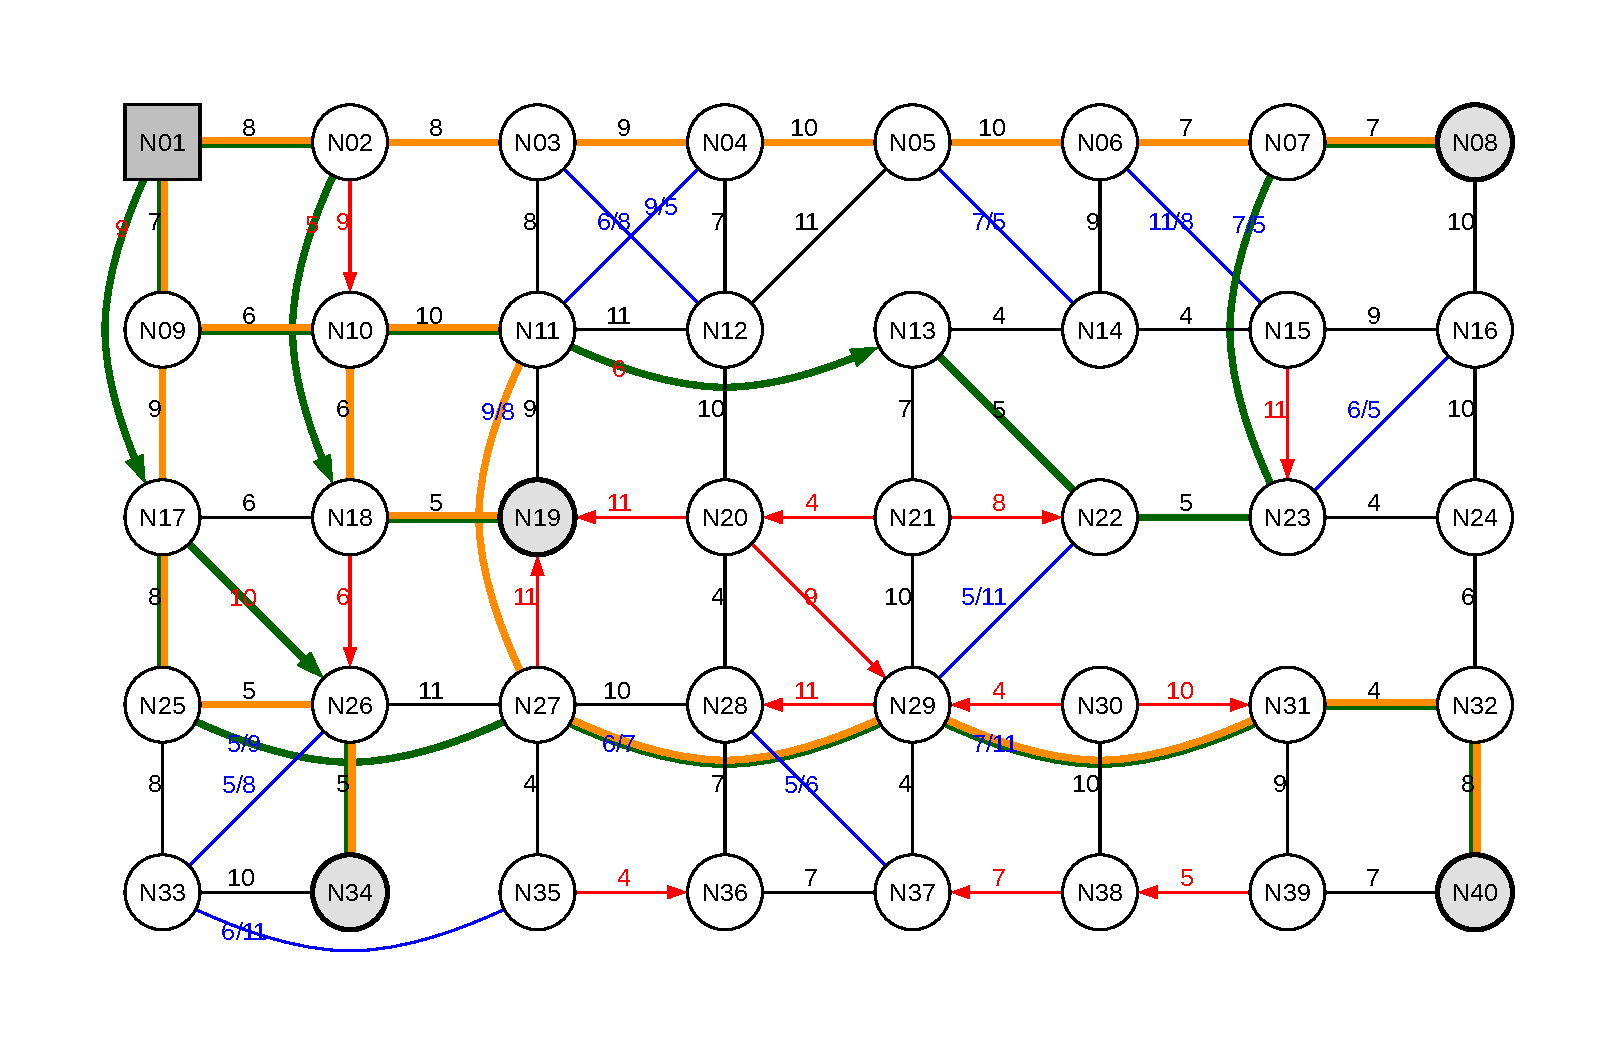
\includegraphics[width=\textwidth]{figuras/grafo_rutas.pdf}
  \caption{Rutas recomendadas por el algoritmo. En verde los tramos de ida y en naranja los de regreso; las líneas dobles son tramos que se usan en ambos sentidos.}
  \label{fig:rutas}
\end{figure}

\section{Descripción del modelo de simulación}

\subsection{Llegada de pedidos y asignación de destinos}

Los pedidos llegan de forma variable con un promedio de $\lambda$ por hora, por lo que se modelaron como un proceso de Poisson: los tiempos entre llegadas son independientes y siguen una distribución exponencial con media $60/\lambda$ minutos (Law, 2015). Cada tiempo se genera con el método de la transformada inversa. Si $U$ es un número uniforme en $(0,1)$, entonces
\begin{equation}
  X = -\frac{60}{\lambda}\,\ln(1-U)
\end{equation}
tiene la distribución exponencial buscada. Las llegadas se acumulan desde el minuto 0 y se detienen cuando la siguiente cae después del cierre de la recepción (480 minutos en una jornada de ocho horas). Para cada pedido se genera además, con el mismo generador, un entero uniforme entre 0 y 3 que indica el destino, de modo que cada zona recibe en promedio la cuarta parte de los pedidos. En 2000 jornadas de prueba se obtuvieron en promedio 32.0, 48.0 y 80.2 pedidos por día con 4, 6 y 10 pedidos por hora, y cada destino recibió entre 24.6\,\% y 25.3\,\% de los pedidos.

\subsection{Eventos, cola y vehículos}

La simulación es de eventos discretos (Banks et al., 2010). Los eventos pendientes se guardan en una lista ordenada por tiempo, implementada con un montículo binario (paquete \texttt{container/heap} de Go), y se procesan uno a la vez:
\begin{itemize}
  \item \textit{Llegada}: si hay un vehículo libre, el pedido sale de inmediato; si no, entra al final de la cola.
  \item \textit{Entrega}: el vehículo llega al destino después del tiempo de ida de su ruta. Se registra la hora de entrega y se programa el regreso.
  \item \textit{Regreso}: el vehículo vuelve a N01 después del tiempo de regreso. Si hay pedidos en cola toma el primero; si no, queda libre.
\end{itemize}
La simulación termina cuando la lista de eventos queda vacía, es decir, cuando se entregó el último pedido y todos los vehículos volvieron a la bodega. Por eso continúa después de las ocho horas cuando todavía quedan pedidos en cola.

\subsection{Políticas comparadas y repeticiones}

En la política actual cada vehículo usa la ruta de las hojas y regresa por el mismo camino; en la política del algoritmo usa la ida y el regreso de Dijkstra. Para que la comparación sea justa se usaron números aleatorios comunes: en cada repetición se genera la lista de pedidos, con sus instantes de llegada y destinos, a partir de una semilla, y esa misma lista se simula con las dos políticas. Así, las diferencias entre ambas corridas se deben solo a las rutas. Se hicieron 10 repeticiones por escenario con las semillas 1 a 10, ocho vehículos y ocho horas de recepción; las mismas semillas se usaron en los barridos de flota y de demanda.

\subsection{Métricas}

Para cada pedido $i$ se registran la hora de solicitud $a_i$, la hora en que sale de la bodega $s_i$ y la hora de entrega $e_i$. La espera es $s_i-a_i$, el tiempo desde la solicitud hasta la entrega es $e_i-a_i$ y el pedido es puntual si $e_i-a_i\le 75$. Si $T$ es la duración de la recepción, $V$ el número de vehículos y $t_{\text{fin}}$ la hora en que vuelve el último vehículo, la utilización de la flota y el tiempo adicional son
\begin{equation}
  U_{\text{flota}} = \frac{\sum_i \left(t^{\text{ida}}_{i} + t^{\text{reg}}_{i}\right)}{V\cdot\max(T,\,t_{\text{fin}})},
  \qquad
  T_{\text{adicional}} = \max\left(0,\ \max_i e_i - T\right).
\end{equation}
Como referencia se calculó también la carga ofrecida
\begin{equation}
  \rho = \frac{\lambda}{60}\cdot\frac{\bar c}{V},
\end{equation}
donde $\bar c$ es el viaje completo promedio de los cuatro destinos (113.5 minutos con las rutas actuales y 79.5 con las de Dijkstra). La carga $\rho$ es la fracción de la flota que en promedio se necesita para atender los pedidos al ritmo en que llegan; si $\rho\ge 1$, los vehículos no alcanzan y la cola crece durante toda la jornada.

\subsection{Verificación}

El programa incluye pruebas automáticas que comprueban los tiempos de las rutas actuales y de Dijkstra, que con 200 vehículos ningún pedido espere y que con la ruta actual ninguna entrega a N40 sea puntual. Además, con una cola en orden de llegada cada pedido sale con el primer vehículo que se desocupa, así que la espera también puede calcularse directamente, pedido por pedido. Para los tres escenarios, la simulación por eventos dio exactamente la misma espera promedio y la misma cantidad de entregas puntuales que ese cálculo directo.

\subsection{Aplicación}

El modelo se programó en Go usando solo la biblioteca estándar. Al ejecutar \texttt{go run .} se inicia un servidor local y la aplicación se abre en el navegador en \url{http://localhost:8080} (Figura~\ref{fig:app}). En ella se elige el escenario (normal, Semana Santa, Navidad o personalizado) y se pueden cambiar el promedio de pedidos por hora, el número de vehículos, la duración de la recepción, la semilla y la cantidad de repeticiones. Al simular, la página muestra el promedio y la desviación estándar de cada métrica para las dos políticas, junto con la carga estimada de la flota.

En la misma página se puede asignar un nuevo tiempo a una conexión, para representar congestión, o cerrarla, en uno o en ambos sentidos, y también restaurar la red original. Cada vez que cambia la red, las rutas del algoritmo se calculan otra vez con Dijkstra sobre la matriz modificada, tanto de ida como de regreso, y la página indica qué rutas cambiaron y cuánto tardan ahora. Las rutas actuales se mantienen; si uno de sus tramos queda cerrado, se reemplaza por el desvío más corto entre sus extremos. Un cambio que deje algún destino sin conexión con la bodega se rechaza. La página dibuja además el grafo con las rutas resaltadas. Los experimentos de este informe se generaron con la opción \texttt{-exportar}, que guarda los resultados en archivos CSV.

\begin{figure}[H]
  \centering
  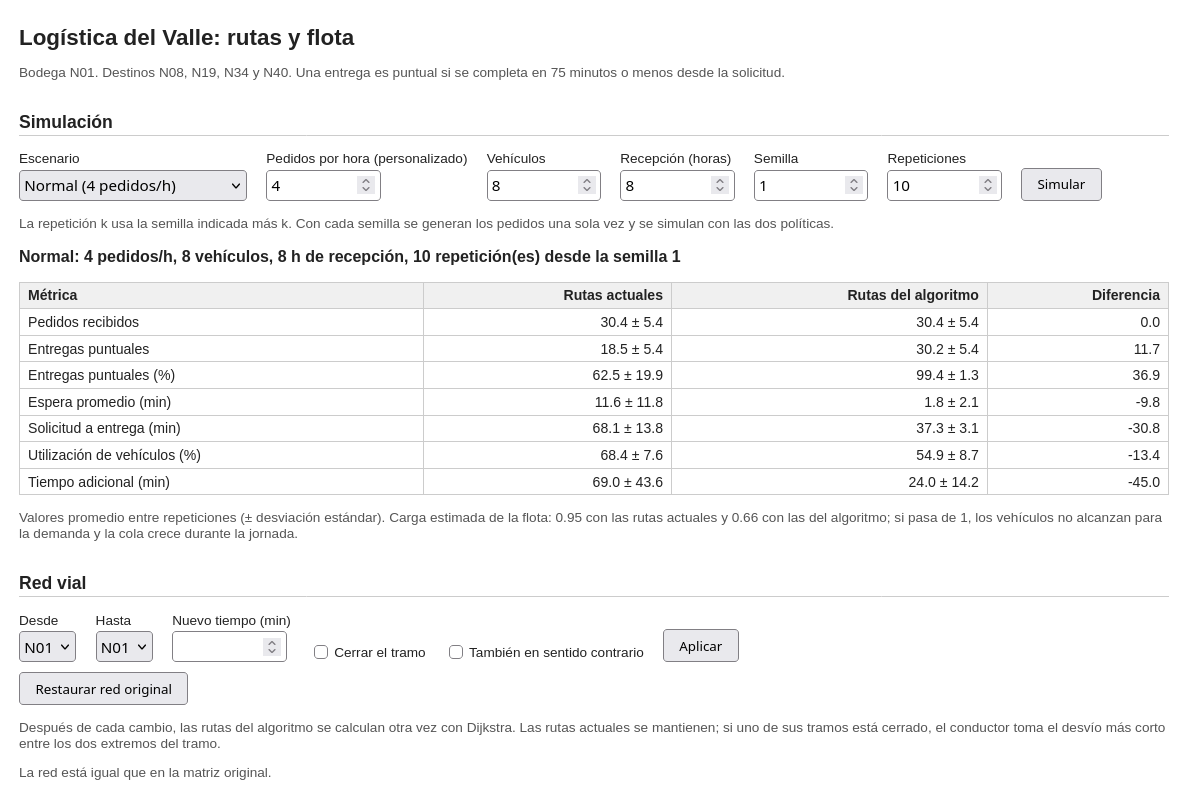
\includegraphics[width=0.85\textwidth]{figuras/aplicacion.png}
  \caption{Parte superior de la aplicación: parámetros de la simulación, resultados del escenario normal con 10 repeticiones y formulario para modificar o cerrar un tramo.}
  \label{fig:app}
\end{figure}

\section{Resultados}

\subsection{Escenarios con la flota actual}

La Tabla~\ref{tab:escenarios} y la Figura~\ref{fig:escenarios} presentan los resultados de las 10 repeticiones de cada escenario con ocho vehículos. En el escenario normal, las rutas del algoritmo elevan las entregas puntuales de 62.5\,\% a 99.4\,\%, reducen la espera promedio de 11.6 a 1.8 minutos y el tiempo hasta la entrega de 68.1 a 37.3 minutos. En Semana Santa la puntualidad pasa de 30.1\,\% a 78.9\,\% y la espera de 70.6 a 17.8 minutos. En Navidad ambas políticas quedan lejos de la meta, con 9.4\,\% y 25.0\,\% de entregas puntuales y esperas promedio de 274.2 y 133.0 minutos. En las 30 parejas de corridas, la política del algoritmo obtuvo un porcentaje de entregas puntuales mayor que la política actual, con diferencias entre 3.6 y 82.2 puntos.

\begin{table}[H]
  \centering
  \footnotesize
  \setlength{\tabcolsep}{4pt}
  \caption{Resultados con ocho vehículos y ocho horas de recepción (media $\pm$ desviación estándar de 10 repeticiones).}
  \label{tab:escenarios}
  \begin{tabular}{l rr rr rr}
    \toprule
    & \multicolumn{2}{c}{Normal} & \multicolumn{2}{c}{Semana Santa} & \multicolumn{2}{c}{Navidad} \\
    \cmidrule(lr){2-3} \cmidrule(lr){4-5} \cmidrule(lr){6-7}
    Métrica & Actual & Algoritmo & Actual & Algoritmo & Actual & Algoritmo \\
    \midrule
    Pedidos recibidos & 30.4 $\pm$ 5.4 & 30.4 $\pm$ 5.4 & 45.3 $\pm$ 6.8 & 45.3 $\pm$ 6.8 & 76.7 $\pm$ 10.0 & 76.7 $\pm$ 10.0 \\
    Entregas puntuales & 18.5 $\pm$ 5.4 & 30.2 $\pm$ 5.4 & 12.7 $\pm$ 7.1 & 34.8 $\pm$ 7.6 & 7.0 $\pm$ 1.5 & 17.9 $\pm$ 7.5 \\
    Entregas puntuales (\%) & 62.5 $\pm$ 19.9 & 99.4 $\pm$ 1.3 & 30.1 $\pm$ 21.1 & 78.9 $\pm$ 20.7 & 9.4 $\pm$ 3.0 & 25.0 $\pm$ 15.1 \\
    Espera promedio (min) & 11.6 $\pm$ 11.8 & 1.8 $\pm$ 2.1 & 70.6 $\pm$ 41.2 & 17.8 $\pm$ 15.4 & 274.2 $\pm$ 75.8 & 133.0 $\pm$ 50.4 \\
    Solicitud a entrega (min) & 68.1 $\pm$ 13.8 & 37.3 $\pm$ 3.1 & 127.2 $\pm$ 42.5 & 53.2 $\pm$ 15.8 & 332.1 $\pm$ 77.1 & 168.7 $\pm$ 51.1 \\
    Utilización (\%) & 68.4 $\pm$ 7.6 & 54.9 $\pm$ 8.7 & 81.3 $\pm$ 4.2 & 75.9 $\pm$ 8.5 & 91.0 $\pm$ 1.4 & 91.0 $\pm$ 1.7 \\
    Tiempo adicional (min) & 69.0 $\pm$ 43.6 & 24.0 $\pm$ 14.2 & 213.1 $\pm$ 92.3 & 60.2 $\pm$ 30.4 & 654.7 $\pm$ 171.3 & 316.5 $\pm$ 113.1 \\
    Carga estimada $\rho$ & 0.95 & 0.66 & 1.42 & 0.99 & 2.36 & 1.66 \\
    \bottomrule
  \end{tabular}
\end{table}

\begin{figure}[H]
  \centering
  \begin{tikzpicture}
    \begin{axis}[barras, ymax=125, ytick={0,25,50,75,100}, ylabel={Entregas puntuales (\%)}]
      \addplot[actual] table[x=idx, y=pct_act, col sep=comma] {datos/resumen.csv};
      \addplot[algoritmo] table[x=idx, y=pct_alg, col sep=comma] {datos/resumen.csv};
    \end{axis}
  \end{tikzpicture}\hfill
  \begin{tikzpicture}
    \begin{axis}[barras, ylabel={Espera promedio (min)}]
      \addplot[actual] table[x=idx, y=espera_act, col sep=comma] {datos/resumen.csv};
      \addplot[algoritmo] table[x=idx, y=espera_alg, col sep=comma] {datos/resumen.csv};
    \end{axis}
  \end{tikzpicture}

  \vspace{0.3cm}
  \begin{tikzpicture}
    \begin{axis}[barras, ymax=125, ytick={0,25,50,75,100}, ylabel={Utilización (\%)}]
      \addplot[actual] table[x=idx, y=util_act, col sep=comma] {datos/resumen.csv};
      \addplot[algoritmo] table[x=idx, y=util_alg, col sep=comma] {datos/resumen.csv};
    \end{axis}
  \end{tikzpicture}\hfill
  \begin{tikzpicture}
    \begin{axis}[barras, ylabel={Tiempo adicional (min)}]
      \addplot[actual] table[x=idx, y=adicional_act, col sep=comma] {datos/resumen.csv};
      \addplot[algoritmo] table[x=idx, y=adicional_alg, col sep=comma] {datos/resumen.csv};
    \end{axis}
  \end{tikzpicture}
  \caption{Promedios por escenario con ocho vehículos. Gris: rutas actuales; azul: rutas del algoritmo.}
  \label{fig:escenarios}
\end{figure}

La utilización es menor con las rutas del algoritmo en los escenarios normal y Semana Santa porque cada pedido ocupa al vehículo menos tiempo: se hace el mismo trabajo con menos horas de vehículo. En Navidad la utilización es de 91\,\% con ambas políticas, porque los vehículos pasan casi toda la operación ocupados; lo que cambia es cuánto se alarga la jornada para terminar los pedidos. El tiempo adicional también muestra el efecto de la cola: en el escenario normal, el último pedido se entrega en promedio 69.0 minutos después del cierre con las rutas actuales y 24.0 con las nuevas, mientras que en Navidad la operación se extiende 10.9 horas con las rutas actuales y 5.3 horas con las del algoritmo.

\subsection{Tamaño de la flota}

La Figura~\ref{fig:flota} muestra el porcentaje de entregas puntuales con 4 a 20 vehículos. Con las rutas del algoritmo se supera el 95\,\% con 7 vehículos en el escenario normal, con 10 en Semana Santa y con 15 en Navidad, y se llega al 100\,\% con 10, 11 y 18 vehículos, respectivamente. Con las rutas actuales la puntualidad nunca pasa de 76.9\,\%: a partir de cierto número de vehículos ya no hay espera, pero los pedidos a N40, que en estas repeticiones son cerca de la cuarta parte, siguen llegando tarde. En Navidad, incluso con 20 vehículos, la política actual se queda en 66.3\,\%.

\begin{figure}[H]
  \centering
  \begin{tikzpicture}
    \begin{axis}[
        width=0.9\textwidth, height=6.5cm,
        xlabel={Número de vehículos}, ylabel={Entregas puntuales (\%)},
        xmin=4, xmax=20, ymin=0, ymax=105, xtick={4,6,...,20}, ytick={0,25,50,75,100},
        grid=major, grid style={gray!25},
        tick label style={font=\footnotesize}, label style={font=\footnotesize},
        legend style={font=\scriptsize, at={(0.5,-0.2)}, anchor=north, legend columns=3, draw=none},
        every axis plot/.append style={thick, mark size=1.4pt, mark options={solid}},
      ]
      \addplot[blue!70!black, mark=*] table[x=vehiculos, y=normal_pct_alg, col sep=comma] {datos/flota.csv};
      \addplot[orange!85!black, mark=square*] table[x=vehiculos, y=santa_pct_alg, col sep=comma] {datos/flota.csv};
      \addplot[red!75!black, mark=triangle*] table[x=vehiculos, y=navidad_pct_alg, col sep=comma] {datos/flota.csv};
      \addplot[blue!70!black, dashed, mark=o] table[x=vehiculos, y=normal_pct_act, col sep=comma] {datos/flota.csv};
      \addplot[orange!85!black, dashed, mark=square] table[x=vehiculos, y=santa_pct_act, col sep=comma] {datos/flota.csv};
      \addplot[red!75!black, dashed, mark=triangle] table[x=vehiculos, y=navidad_pct_act, col sep=comma] {datos/flota.csv};
      \draw[dotted, thick] (axis cs:8,0) -- (axis cs:8,105);
      \legend{Normal (algoritmo), Semana Santa (algoritmo), Navidad (algoritmo),
        Normal (actual), Semana Santa (actual), Navidad (actual)}
    \end{axis}
  \end{tikzpicture}
  \caption{Entregas puntuales según el número de vehículos (promedio de 10 repeticiones). Líneas continuas: rutas del algoritmo; discontinuas: rutas actuales. La línea punteada marca la flota actual de ocho vehículos.}
  \label{fig:flota}
\end{figure}

\subsection{Aumento de la demanda}

La Figura~\ref{fig:demanda} muestra qué ocurre con ocho vehículos cuando el promedio de pedidos va de 1 a 12 por hora. Con las rutas del algoritmo la puntualidad se mantiene por encima de 94\,\% hasta 5 pedidos por hora y cae a 78.9\,\% con 6, a 42.8\,\% con 8 y a 25.0\,\% con 10. Con las rutas actuales nunca supera 76\,\%, aun con muy pocos pedidos, y cae a partir de 4 pedidos por hora; con 6 pedidos por hora ya está en 30.1\,\%. La espera crece mucho más rápido con las rutas actuales: con 8 pedidos por hora es de 169.3 minutos, contra 66.9 con las rutas del algoritmo.

\begin{figure}[H]
  \centering
  \begin{tikzpicture}
    \begin{axis}[
        width=0.48\textwidth, height=5.5cm,
        xlabel={Pedidos por hora}, ylabel={Entregas puntuales (\%)},
        xmin=1, xmax=12, ymin=0, ymax=105, xtick={2,4,...,12}, ytick={0,25,50,75,100},
        grid=major, grid style={gray!25},
        tick label style={font=\footnotesize}, label style={font=\footnotesize},
        legend style={font=\scriptsize, at={(0.97,0.97)}, anchor=north east},
        every axis plot/.append style={thick, mark size=1.4pt, mark options={solid}},
      ]
      \addplot[blue!55!black, mark=*] table[x=porhora, y=pct_alg, col sep=comma] {datos/demanda.csv};
      \addplot[gray!60!black, dashed, mark=o] table[x=porhora, y=pct_act, col sep=comma] {datos/demanda.csv};
      \draw[dotted] (axis cs:4,0) -- (axis cs:4,105);
      \draw[dotted] (axis cs:6,0) -- (axis cs:6,105);
      \draw[dotted] (axis cs:10,0) -- (axis cs:10,105);
      \legend{Algoritmo, Actual}
    \end{axis}
  \end{tikzpicture}\hfill
  \begin{tikzpicture}
    \begin{axis}[
        width=0.48\textwidth, height=5.5cm,
        xlabel={Pedidos por hora}, ylabel={Espera promedio (min)},
        xmin=1, xmax=12, ymin=0, xtick={2,4,...,12},
        grid=major, grid style={gray!25},
        tick label style={font=\footnotesize}, label style={font=\footnotesize},
        every axis plot/.append style={thick, mark size=1.4pt, mark options={solid}},
      ]
      \addplot[blue!55!black, mark=*] table[x=porhora, y=espera_alg, col sep=comma] {datos/demanda.csv};
      \addplot[gray!60!black, dashed, mark=o] table[x=porhora, y=espera_act, col sep=comma] {datos/demanda.csv};
    \end{axis}
  \end{tikzpicture}
  \caption{Efecto de la demanda con ocho vehículos (promedio de 10 repeticiones). Las líneas punteadas marcan los escenarios normal, Semana Santa y Navidad (4, 6 y 10 pedidos por hora).}
  \label{fig:demanda}
\end{figure}

\subsection{Cierre de un tramo}

Como ejemplo de incidente vial se cerró la calle N17--N25 en ambos sentidos. Con la política actual, la ruta a N34 pierde ese tramo y el conductor toma desvíos: la ida pasa a ser N01, N09, N17, N26, N25, N33, N34 (49 minutos) y el regreso N34, N33, N25, N27, N19, N18, N17, N09, N01 (61 minutos), porque N26$\rightarrow$N17 no existe y el camino más corto de N25 a N17 da una vuelta larga. Con el algoritmo, Dijkstra cambia dos rutas: el regreso desde N34 pasa a N34, N26, N25, N27, N11, N10, N09, N01 (46 minutos en lugar de 34) y la ida a N40 a N01, N17, N26, N25, N27, N29, N31, N32, N40 (54 minutos en lugar de 47). Las demás rutas no cambian. La Tabla~\ref{tab:cierre} compara los resultados con los de la red original.

\begin{table}[H]
  \centering
  \small
  \caption{Efecto del cierre de N17--N25 con ocho vehículos (promedio de 10 repeticiones).}
  \label{tab:cierre}
  \begin{tabular}{l l rr rr rr}
    \toprule
    & & \multicolumn{2}{c}{Puntuales (\%)} & \multicolumn{2}{c}{Espera (min)} & \multicolumn{2}{c}{Carga $\rho$} \\
    \cmidrule(lr){3-4} \cmidrule(lr){5-6} \cmidrule(lr){7-8}
    Escenario & Política & Original & Cierre & Original & Cierre & Original & Cierre \\
    \midrule
    Normal & Actual & 62.5 & 56.9 & 11.6 & 16.6 & 0.95 & 1.00 \\
           & Algoritmo & 99.4 & 98.8 & 1.8 & 2.3 & 0.66 & 0.70 \\
    Semana Santa & Actual & 30.1 & 24.2 & 70.6 & 86.3 & 1.42 & 1.50 \\
           & Algoritmo & 78.9 & 70.8 & 17.8 & 23.7 & 0.99 & 1.05 \\
    Navidad & Actual & 9.4 & 8.9 & 274.2 & 305.5 & 2.36 & 2.50 \\
           & Algoritmo & 25.0 & 20.6 & 133.0 & 154.0 & 1.66 & 1.76 \\
    \bottomrule
  \end{tabular}
\end{table}

\section{Discusión}

Cambiar las rutas es la medida con mayor efecto y no requiere vehículos adicionales. El viaje completo promedio baja de 113.5 a 79.5 minutos, y eso actúa por dos vías. La primera es directa: con idas más cortas hay más margen para esperar y, en particular, los pedidos a N40 pasan de ser siempre tardíos a poder entregarse a tiempo. La segunda es la capacidad: si cada viaje dura menos, los vehículos vuelven antes, la carga de la flota baja de 0.95 a 0.66 en el escenario normal y la cola casi desaparece. Con las mismas condiciones, la puntualidad mejora 36.9 puntos en el escenario normal, 48.8 en Semana Santa y 15.6 en Navidad, y el tiempo adicional se reduce entre 52\,\% y 72\,\%.

Al aumentar la demanda, la carga crece en proporción al número de pedidos. Con ocho vehículos, $\rho=1$ se alcanza con unos $60\cdot 8/113.5\approx 4.2$ pedidos por hora usando las rutas actuales y con unos $60\cdot 8/79.5\approx 6.0$ usando las del algoritmo. Esto coincide con la Figura~\ref{fig:demanda}: la política actual empieza a deteriorarse ya en el escenario normal, y la del algoritmo se mantiene bien hasta 5 pedidos por hora y empieza a fallar en Semana Santa, que con $\rho=0.99$ queda justo en el límite. En Navidad la carga supera 1 con ambas políticas y la cola crece durante toda la jornada, lo que explica esperas de varias horas y la variabilidad alta entre repeticiones: los días con más pedidos acumulan una cola mucho mayor.

La cantidad de vehículos se vuelve una limitación cuando $\rho$ se acerca a 1. Para que $\rho<1$ se necesitan al menos 8, 12 y 19 vehículos con las rutas actuales, y 6, 8 y 14 con las del algoritmo, en los escenarios normal, Semana Santa y Navidad. Esa condición evita que la cola crezca sin control, pero no garantiza la puntualidad; según el barrido de flota, para superar el 95\,\% de entregas puntuales con las rutas del algoritmo se necesitan 7, 10 y 15 vehículos. Con las rutas actuales ningún tamaño de flota alcanza esa meta, porque el límite lo pone la ruta a N40 y no la cantidad de vehículos. Así, la flota de ocho vehículos es suficiente en un día normal solo si se cambian las rutas; en Semana Santa hacen falta al menos dos vehículos más y en Navidad cerca del doble.

El cierre de N17--N25 afecta de forma distinta a cada política. En el escenario normal, la política actual pierde 5.6 puntos de puntualidad, porque el desvío de N34 alarga la ida 7 minutos y el regreso 19 y su carga llega a 1.00; la del algoritmo reorganiza las rutas y pierde solo 0.6 puntos. En Semana Santa ocurre lo contrario: la política del algoritmo pierde 8.1 puntos frente a 5.9 de la actual, porque el cierre lleva su carga de 0.99 a 1.05 y la flota pasa a estar saturada. En Navidad las dos políticas ya estaban saturadas antes del cierre. Aun así, en los tres escenarios las rutas recalculadas siguen dando mejores resultados que las actuales.

La simulación no representa varios aspectos de la operación real. Los tiempos de viaje son fijos, cuando en la práctica dependen del tráfico y de la hora. No se incluyen el tiempo de carga y entrega, los descansos, los turnos, las averías ni la posibilidad de llevar varios pedidos a la misma zona en un solo viaje. Se supone además que los pedidos llegan a un ritmo constante durante el día, sin horas pico, y que las cuatro zonas se reparten la demanda por igual; cada zona se trata como un punto, aunque en realidad incluye varias direcciones. Los cierres de tramos duran toda la jornada y no se consideran costos de combustible ni de personal. Finalmente, los resultados dependen de que la matriz refleje los tiempos actuales de la red.

\section{Conclusiones}

\begin{enumerate}
  \item La red es un grafo dirigido de 40 nodos y 144 arcos, con 18 calles de un solo sentido. Las cuatro rutas de las hojas de despacho son válidas de ida y de regreso, por lo que la instrucción de volver por el mismo camino puede cumplirse; sin embargo, la ida a N40 tarda 93 minutos y hace imposible que esas entregas sean puntuales.
  \item Las rutas de Dijkstra reducen la ida en los cuatro destinos (de 59, 33, 42 y 93 minutos a 51, 18, 24 y 47) y el viaje completo promedio en 30\,\%. El regreso debe planificarse por separado, porque las idas óptimas usan calles de un solo sentido y no pueden recorrerse al revés.
  \item Con los mismos pedidos, las rutas del algoritmo elevan la puntualidad de 62.5\,\% a 99.4\,\% en el escenario normal, de 30.1\,\% a 78.9\,\% en Semana Santa y de 9.4\,\% a 25.0\,\% en Navidad, y reducen a menos de la mitad la espera y el tiempo adicional para terminar los pedidos.
  \item Con ocho vehículos la flota alcanza para un día normal solo con las nuevas rutas. En Semana Santa trabaja al límite y en Navidad es insuficiente: para superar el 95\,\% de entregas puntuales con las rutas del algoritmo se necesitan alrededor de 10 vehículos en Semana Santa y 15 en Navidad.
\end{enumerate}

\subsection*{Reflexión final}

Para la empresa, el cambio con mayor impacto y menor costo es actualizar las hojas de despacho con rutas de ida y de regreso distintas, ya que mejora la puntualidad y reduce las horas extra sin comprar vehículos. Para las temporadas altas, el modelo indica que no basta con las rutas, y que conviene planificar con anticipación vehículos adicionales o temporales, en especial para Navidad. La aplicación permite repetir este análisis cuando cambie la demanda o cuando se cierre o congestione una calle, antes de tomar la decisión en la operación real.

Estos resultados deben tomarse con cautela antes de aplicarlos. El modelo usa tiempos fijos, entregas instantáneas y una demanda uniforme, y no considera horarios de trabajo ni costos. Antes de cambiar las rutas convendría medir los tiempos reales de los nuevos recorridos, revisar con los conductores que las calles de un solo sentido se usen como indica la matriz y hacer una prueba piloto en uno o dos destinos.

\section*{Referencias}

\begin{list}{}{\setlength{\leftmargin}{1.27cm}\setlength{\itemindent}{-1.27cm}\setlength{\itemsep}{0.3em}}
  \item Banks, J., Carson, J. S., Nelson, B. L. y Nicol, D. M. (2010). \textit{Discrete-event system simulation} (5.ª ed.). Pearson.
  \item Bellman, R. (1958). On a routing problem. \textit{Quarterly of Applied Mathematics, 16}(1), 87--90. \url{https://doi.org/10.1090/qam/102435}
  \item Cormen, T. H., Leiserson, C. E., Rivest, R. L. y Stein, C. (2022). \textit{Introduction to algorithms} (4.ª ed.). MIT Press.
  \item Dijkstra, E. W. (1959). A note on two problems in connexion with graphs. \textit{Numerische Mathematik, 1}, 269--271. \url{https://doi.org/10.1007/BF01386390}
  \item Floyd, R. W. (1962). Algorithm 97: Shortest path. \textit{Communications of the ACM, 5}(6), 345. \url{https://doi.org/10.1145/367766.368168}
  \item Gansner, E. R. y North, S. C. (2000). An open graph visualization system and its applications to software engineering. \textit{Software: Practice and Experience, 30}(11), 1203--1233. \url{https://doi.org/10.1002/1097-024X(200009)30:11<1203::AID-SPE338>3.0.CO;2-N}
  \item Hart, P. E., Nilsson, N. J. y Raphael, B. (1968). A formal basis for the heuristic determination of minimum cost paths. \textit{IEEE Transactions on Systems Science and Cybernetics, 4}(2), 100--107. \url{https://doi.org/10.1109/TSSC.1968.300136}
  \item Law, A. M. (2015). \textit{Simulation modeling and analysis} (5.ª ed.). McGraw-Hill Education.
\end{list}

\end{document}
